% \paragraph{Problem Formulation.} 

Our work focuses on the {\it median} of the equilibrium
opinion vector (or simply, the median opinion),
which we defined in Equation~\eqref{eq:fj2}.
The median opinion indicates exactly where
the majority lies, and therefore directly
relates to winning or loosing an election.
In this section, we introduce different
strategies that can be used to optimize
the median in a specific direction.
%
For simplicity, we only
formally provide an objective with the goal to
maximize the median, but the minimization
objective can be defined analogously.
%
We introduce the following optimization problem
where we want to maximize the increase in the
median opinion under a fixed budget $k$ of the resistance parameter change. 
For any agent $u \in V$, we may change
its resistance $\alpha_u$, but not its
innate opinion $s_u$; this reflects a simple
attack on someone's susceptibility to persuasion
\cite{abebe2020opinion}.
%
We measure distances between the original
resistance vector $\alpha$ and modified
resistances $\alpha'$ in an arbitrary
$\ell_p$ norm $\| \cdot \|_p$, and we obtain
one optimization problem for each value
of $p \ge 0$.

\begin{tcolorbox}
\begin{problem}[\textsc{Maximizing the Median under FJ Dynamics}]
\label{prob:max-median} Let $(\alpha, W, s)$ be a network
of generalized FJ dynamics and $k$ be a budget on the change of resistance values. Maximize the objective
$\mathrm{Median}(x^\star(\alpha', W, s))$
where $\alpha' \in [0,1]^n$ is a vector of resistances
such that $\|\alpha' - \alpha\|_p \le k$

%where $\| \cdot \|_p$ denotes the $\ell_p$ norm.
\end{problem}
\end{tcolorbox}


We also consider the dual of this problem, which
addresses the question of how many stooges are
needed in order to flip the median beyond
a certain threshold $\theta$. This problem directly addresses the question of what budget is necessary in order to win an election. 

\begin{tcolorbox}
\begin{problem}[\textsc{Flipping the Median under FJ Dynamics}]
\label{prob:elections}
Let $(\alpha, W, s)$ be a network of generalized FJ dynamics
and $\theta \in \R$ a threshold.
Minimize $\|\alpha' - \alpha\|_p$ such that
$\alpha' \in [0,1]^n$ is a vector of resistances
with $\mathrm{Median}(x^\star(\alpha, W, s)) > \theta$.
\end{problem}
\end{tcolorbox}


The two norms of interest in this work are for $p\in\{0,1\}$. The $\ell_0$
pseudo-norm is defined as
$\| \alpha - \alpha' \|_0 = |\{ u \in V : \alpha_u \not= \alpha'_u \}|$
which counts the number of distinct elements.
This corresponds to targeting
$k$ nodes and converting them into stooges. The variant with $p=1$ has also received attention in the literature~\cite{chan2021hardness}. 


\begin{figure}
    \centering
    \small
    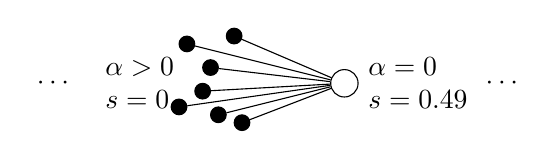
\begin{tikzpicture}
        \node at (-1.7, -0.5) {$\cdots$};
        \node at (4, -0.5) {$\cdots$};
        \node[align=left] at (-0.6, -0.5) {$\alpha>0$\\ $s=0$};
        \node[inner sep=2pt, draw=black, circle, fill] (u1) at (0, 0) {};
        \node[inner sep=2pt, draw=black, circle, fill] (u2) at (0.6, 0.1) {};
        \node[inner sep=2pt, draw=black, circle, fill] (u3) at (-0.1, -0.8) {};
        \node[inner sep=2pt, draw=black, circle, fill] (u4) at (0.3, -0.3) {};
        \node[inner sep=2pt, draw=black, circle, fill] (u5) at (0.2, -0.6) {};
        \node[inner sep=2pt, draw=black, circle, fill] (u6) at (0.4, -0.9) {};
        \node[inner sep=2pt, draw=black, circle, fill] (u7) at (0.7, -1) {};
        \node[inner sep=3.5pt, draw=black, circle, label={[align=left]right:$\alpha=0$\\ $s=0.49$}] (v) at (2, -0.5) {};
        \draw (u1) to (v);
        \draw (u2) to (v);
        \draw (u3) to (v);
        \draw (u4) to (v);
        \draw (u5) to (v);
        \draw (u6) to (v);
        \draw (u7) to (v);
    \end{tikzpicture}
    \caption{An example showcasing challenges in
    Problems~\ref{prob:max-median}
    and \ref{prob:elections}. We show
    an isolated component in a larger
    graph, where the black vertices
    on the left have innate innate opinion
    $0$, but are only connected to the
    white vertex on the right with innate
    opinion $0.5$ but resistance $0$.}
    \label{fig:example}
\end{figure}

We can trivially convert an algorithm for
Problem~\ref{prob:max-median} into an
algorithm addressing Problem~\ref{prob:elections}
by a binary search over the budgets.
%
A natural heuristic for these optimization
problems is the greedy algorithm, which
in each iteration designates a new node
as a stooge, and the selection is made 
such that it maximizes the increase in the
median opinion.
%
This solves both problems at the same time,
as we can keep adding stooges until we
flip the median opinion across the
threshold $\theta$.
%
However, Figure~\ref{fig:example} exemplifies
a difficulty with this approach:
Initially, it may seem that using the
the white node on the right as a stooge
and changing its resistance to $\alpha=1$
results in a big increase in the
median opinions. However,
if the objective is to move the
median beyond a threshold of $\theta=0.5$,
this modification is in vain, since it
does not move any opinion past the
threshold. Furthermore, employing
more stooges in the shown isolated
component does not help with our objective either.
%
Greedily selecting stooges is therefore
problematic. Other problems with
the greedy algorithm are its inefficiency
on large graphs, since we need to identify
the best node to become a stooge in
each iteration. We will later
discuss the greedy algorithm and how to
apply it on large networks.
We show formally that our targeted
problems are hard to approximate in
Theorem~\ref{thm:hardness}.
In the remainder of this section,
we analyze the hardness and discuss different heuristics
to address Problems~\ref{prob:max-median}
and Problem~\ref{prob:elections}.

\subsection{Hardness of Problem~\ref{prob:max-median}}

Our first key result is that Problem~\ref{prob:max-median} is computationally hard. Specifically, we establish the following inapproximability result. 

\begin{theorem}
    \label{thm:hardness}
    Problem~\ref{prob:max-median}
    for $p=0$
    is inapproximable
    to any multiplicative factor
    unless $\mathsf{P} = \mathsf{NP}$.
\end{theorem}


The proof is based on a novel reduction from the set cover problem~\cite{williamson2011design}, which we defer to the appendix. Furthermore, a straight-forward corollary of our reduction shows that this result carries over not only to the $\frac{1}{2}$-percentile which is the median, but to any $q$-quantile for $0 < q < 1$.

\begin{corollary}
\label{cor:quantile}
Let $(\alpha, W, s)$ be a network of generalized FJ  dynamics,
let $k$ be a budget and $0 < q < 1$  be any fixed quantile value.
The problem of maximizing the $q$-th quantile of $x^\star(\alpha', W, s)$ subject to $\|\alpha' - \alpha\|_0 \le k$ (akin to Problem~\ref{prob:max-median} for $q=\frac{1}{2}$) cannot be approximated to any multiplicative factor unless $\mathsf{P} = \mathsf{NP}$.
\end{corollary}

On the other hand,
for the special case of directed trees,
we can solve this problem optimally
in polynomial time using dynamic programming,
which we show in the appendix.


\subsection{Huber M-Estimator}



To circumvent the hardness of
maximizing the median
and avoid the aforementioned
issues with the greedy algorithm,
we want to turn our attention on
a continuous approximation of the median which
makes our objectives amenable to iterative methods.
The median as a function represents a piecewise-defined
function characterized by inherent discontinuities.
This non-differentiable nature precludes the applicability
of gradient-based optimization techniques, which
fundamentally rely on smooth and continuous objectives
to ensure convergence towards a (potentially locally)
optimal solution. 
Continuous approaches do not commit
to stooges, which could lead to problems as the one
shown in Figure~\ref{fig:example}.
Our approach for tackling Problem~\ref{prob:elections} is
formally stated in Algorithm~\ref{alg:huber-gd}.
However, before delving into details, we
want to motivate our continuous relaxation. We start by
using the Huber M-estimator to derive smooth,
differentiable formulations for the median,
akin to how the softmax function serves as a smooth
approximation for the maximum value
\cite{brown2001smoothed,hampel2011smoothing}.
The Huber M-estimator is a robust statistical estimator that
combines properties of both the sample mean and the sample
median to produce an estimate that is resistant to outliers.
The key idea is to minimize a function of residuals that is
quadratic for small residuals but linear for large residuals.
The Huber loss is parameterized by a tuning constant $c$ and is defined as 
\[
    H_c(x) =
    \begin{cases} 
        \frac 1 2 x^2 & \textrm{if } |x| \le c \\
        c \cdot \left(|x| - \frac 1 2 c\right) & \textrm{otherwise} .
    \end{cases} 
\]
%
The tuning constant $c$ determines the point at which the loss switches from being quadratic to linear. The intuition behind Huber's M-estimator being a good proxy for the median lies in its loss function, which is less sensitive to outliers than the mean. The mean averages all values equally, giving high influence to outliers, while the median is resistant to outliers but does not take into account ``how far'' the other points are from it.  To find Huber's M-estimator $\hat y$ for a data set \( \{ x_1, x_2, \ldots, x_n \} \), we
solve the minimization
\begin{align}
    \label{eq:y-star}
    \hat y = \hat y_c = \min_y \sum_{i=1}^{n} H_c(x_i - y) .
\end{align}
The extreme values of $c$
give us either the median or
the mean, as $\hat y_0 = \mathrm{Median}(\bx)$
and $\hat y_\infty = \mathrm{Mean}(\bx)$. After introducing the robust and continuous
approximation to the median, we now state a continuous adaption of
Problem~\ref{prob:elections} with $\ell_1$ budget constraint~\cite{chan2021hardness}


%
\begin{formulation}[\textsc{Minimal Budget for Election Influence via FJ Dynamics}]
\label{prob:elections_formal} 
Consider a network of FJ dynamics represented by $(\alpha, W, s)$, where $c \ge 0$ is the Huber loss parameter, and $\theta \in \R$ represents a threshold.  Minimize $\|\alpha' - \alpha\|_1$, subject to the condition that $\alpha' \in [0, 1]^n$ is a vector of resistances, and $\hat y(\alpha') \ge \theta$, where $\hat y(\alpha')$ is defined as $\min_y \sum_{i=1}^n H_c(x^\star_i(\alpha', W, s) - y)$.



% Given an FJ opinion dynamic and ,
% how many nodes do we have to make stooges
% such that $\min_y \sum_i H_c(x_i - y) > \frac 1 2$, where
% $\bx$ are the equilibrium opinions?
% \fabian{we need to use $\|\alpha' - \alpha\|_1$
% as budget for the continuous approaches. How about:
% Let $(\alpha, W, s)$ be a network of FJ dynamics, and
% $\theta \in \R$ a threshold. Minimize
% $\|\alpha' - \alpha\|_1$ such that
% $\alpha' \in [0, 1]^n$ is a vector of resistances
% with $\hat y(\alpha') \ge \theta$
% where $\hat y(\alpha') = \min_y \sum_{i=1}^n H_c(x^\star_i(\alpha', W, s) - y)$.}
\end{formulation}

\iffalse
\spara{Greedy does not work well using Huber's loss.} \labis{visualization will help here? O/w define left, right}
We could try an algorithm that greedily
chooses stooges in order to maximize $H_c(\bx)$.
However, such an algorithm may perform
poorly, at least in theory.
Imagine a large opinion dynamic, where
a $K_{k, n, 1}$ is an isolated tripartite
graph with $n \gg k \gg 1$. The left vertices have resistance
$1$, the middle vertices resistance $\approx 0$,
and the right vertex resistance $1$.
The innate opinions are $0$ for all vertices.
Now, choosing the right vertex 
changes the equilibrium opinions to
$\frac 1 2$ for the $n$ nodes in the middle.
This gives us a potentially big increase in
the mean, and potentially in the median
depending on the rest of the graph.
However, we will never be able to push
a substantial number of the $n$ middle
vertices beyond an opinion of $\frac 1 2$.
Thus, this increase was meaningless
and we should not have picked the right vertex,
but some other vertex in the remainder
of the graph.
\fabian{I think this could also serve
as an example why Problems 2 and 3 are
hard. We could move this ahead and
just state here that we also get an increase
in the mean, so the approx. objective
with huber's loss cannot overcome this
issue. Also, what purpose do the $k$
vertices on the left serve?}
\fi

\paragraph{Gradient Formulation}
We now show how to derive a gradient
for the Huber's M-estimator $\hat y$.
Since the M-Estimator itself is the
result of optimization problem in
Equation~\ref{eq:y-star},
we first need to analyze properties
of the minimizer.
To this end,
we define the set
$I = \{i : |x^\star_i - \hat y| < c\}$.
For any $y \in \mathbb R$,
\[
    \sum_{i} H_c(x^\star_{i} - y) =
    c \sum_{i \notin I} \left(|x^\star_i - y| - \frac 1 2 c\right)
    + \frac 1 2 \sum_{i \in I} (x^\star_i - y)^2
\]
and we thus have the identity
\begin{multline*}
    0 = \frac{\partial}{\partial \hat y} \sum_i H_c(x^\star_i - \hat y)
    = -c \sum_{i \notin I} \mathrm{sgn}(x^\star_i - \hat y)
    - \sum_{i \in I} (x^\star_i - \hat y) \\
    \iff
    \hat y = \frac 1 {|I|} \Big(
      c \sum_{i \notin I} \mathrm{sgn}(x^\star_i - \hat y) +
      \sum_{i \in I} x^\star_i \Big) .
\end{multline*}
Assuming $x^\star_i \not= \hat y$ for all $i$, we thus obtain
\[
    \frac{\partial \hat y}{\partial x^\star_i} =
    \frac 1 {|I|} 1_{[i \in I]}
\]
where we denote with $1_{[\mathrm{cond}(u)]} \in \R^n$
the vector which is $1$ in the rows corresponding
to $u$ where $\mathrm{cond}(u)$ is true and $0$, otherwise.
%
It remains to compute the derivative          \def\transMatrix{W}
$ \partial \bx^\star / \partial \alpha $
where $\bx^\star = (I - (I - A) \transMatrix)^+ A \bs$ are the equilibrium opinions and
$A = \mathrm{Diag}(\alpha)$.
Let
\begin{align*}
    X =
    I - (I - A) \transMatrix
    \quad\textrm{and}\quad
    \bx^\star =
    X^+ A \bs .
\end{align*}
Note that we can obtain $\bx^\star$ without
computing the full pseudoinverse $X^+$
by solving the least-squares problem
$\min_\bx \| X \bx - A \bs \|_2$.
We want to show that
\[
    \frac{\partial \bx^\star}{\partial \alpha} =
    X^+ \mathrm{Diag}(\bs) - X^+ \mathrm{Diag}(\transMatrix \bx^\star) .
\]
By the product rule,
\[
    \frac{\partial \bx^\star}{\partial \alpha} =
    \frac{\partial X^+ A \bs}{\partial \alpha} =
    X^+ \otimes \frac{A \bs}{\partial \alpha} +
    \frac{\partial X^+}{\partial \alpha} \otimes A \bs .
\]
We evaluate both terms. The first term is easy:
\[
    X^+ \otimes \frac{\partial A \bs}{\partial \alpha} =
    X^+ \otimes \mathrm{Diag}(\bs) =
    X^+ \mathrm{Diag}(\bs) .
\]
For the second term, we apply the chain rule:
\[
    \frac{\partial X^+}{\partial \alpha} =
    \frac{\partial X^+}{\partial X} \otimes
    \frac{\partial X}{\partial \alpha} =
    \frac{\partial X^+}{\partial X} \otimes
    \frac{\partial A \transMatrix}{\partial \alpha} .
\]
We  use that
$\partial X^+_{ij} / \partial L_{ab} = -X^+_{ia} X^+_{bj}$
since $X$ has full rank.
Furthermore, 
\[
    \frac{\partial (AM)_{ab}}{\partial a_k}
    = 1_{[a = k]} M_{ab} .
\]
Thus,
\begin{align*}
    \left( \frac{\partial X^+}{\partial X} \otimes
    \frac{\partial A \transMatrix}{\partial \alpha} \right)_{ijk}
    &= - \sum_{a,b} X^+_{ia} X^+_{bj} 1_{[a = k]} M_{ab} \\
    &= - \sum_{b} X^+_{ik} X^+_{bj} M_{kb}
    = - X^+_{ik} (\transMatrix X^+)_{kj}
\end{align*}
and
\begin{align*}
    \left( \frac{\partial X^+}{\partial \alpha} \otimes A \bs \right)_{ik} &=
    - \sum_j X^+_{ik} (\transMatrix X^+)_{kj} (A \bs)_j \\ &=
    - X^+_{ik} (\transMatrix X^+ A \bs)_{k} =
    - X^+_{ik} (\transMatrix x^\star)_{k}
\end{align*}
which means
$\partial X^+ / \partial \alpha \otimes A \bs = - X^+ \mathrm{Diag}(\transMatrix \bx^\star)$.
%
Putting everything together, we get
\begin{align}
    \label{eq:2}
    \nabla \hat y &= \frac 1 {|I|}
        \mathrm{Diag}(\bs - \transMatrix \bx^\star) (X^+)^\top 1_{[i \in I]}
\end{align}
which we can again solve efficiently by solving
the last squares problem
$\min_{z} \| X^\top z - 1_{[i \in I]} \|_2$.
Then, assuming $z$ is the solution
to the least squares problem,
we have that
$\nabla \hat y = \frac 1 {|I|} \mathrm{Diag}(\bs - \transMatrix \bx) z$.



\begin{algorithm}
\caption{Optimizing $\hat y$ with Gradient Ascent}
\label{alg:huber-gd}
\begin{algorithmic}[1]
\Function{Projected Huber}{$W, \alpha_0, s, k, \eta$}
    \State $\alpha \gets \alpha_0$
    \While{not converged}
        \State Let $X = I - (I - A) \transMatrix$ where $A = \mathrm{Diag}(\alpha)$
        \State Solve $\bx^\star = \min_{\bx} \| X \bx - A \bs \|_2$
        \com{Calculate opinions}
        \State Let $\hat y = \min_{y} \sum_i H_c (x^\star_i - y)$
        \com{Huber M-estimator}
        \State Let $I = \{ i : |x^\star_i - \hat y| < c \}$
        \State Solve $\hat z = \min_{z} \|X^\top z - 1_{[i \in I]}\|_2$
        \State Let $\nabla \hat y = \frac 1 {|I|} \mathrm{Diag}(\bs - \transMatrix \bx) \hat z$
        \com{Determine gradient}
        \State $\alpha' \gets \alpha + \eta \nabla \hat y$
        \com{Gradient update}
        \State $\alpha \gets \min \{ \|\alpha - \alpha'\|_2 :
            \|\alpha - \alpha_0\|_1 \le k \}$
        \com{Projection}
    \EndWhile
    \State \Return $\alpha$
\EndFunction
\end{algorithmic}
\end{algorithm}


\spara{Algorithm and complexity}
We optimize the robust median $\hat y$
via gradient ascent with step size
$\eta > 0$, as shown in
Algorithm~\ref{alg:huber-gd}.
%
For a single gradient computation, we need to
solve the two least squares problems to obtain
$\bx$ via Equation~\eqref{eq:fj2} and
$\nabla \hat y$ via Equation~\ref{eq:2}.
We further carry out a constant number of
matrix multiplications, where each matrix
is of size $n$. In total, a single gradient
computation thus has worst-case running
time $O(n^3)$.

\spara{Selecting the Huber tuning constant $c$}
Our continuous optimization via the Huber
M-Estimator relies on a good choice of
$c$. Generally, this choice is instance-specific
and involves a trade-off between robustness
and approximation quality of the median.
Choosing a value of $c$
that is too small may introduce issues
with vanishing gradients.
We will later give an approach to set an
appropriate value of $c$ in our experiments
in Section~\ref{sec:exp}.

\iffalse
In contrast, each evaluation of the marginal gain
in greedy is just as expensive asymptotically
(as it also involves solving a linear system). However,
this can be sped up by computing $\bx$ via simulation
which can warm start using the equilibirum opinions
of the previous iteration. Overall, we compute
$O(B n)$ marginal gains where $B$ is the
number of stooges.
\fi


\subsection{Sigmoid Threshold Influence Method}
\label{sec:sigmoid}

We consider a second natural method
for the continuous objective.
However, this method is only suited
to flip the median, as defined in
Problem~\ref{prob:elections_formal}.
Here, we create an objective
that rewards opinions above $\theta$
and penalizes opinions below $\theta$.
Imagine an objective that is simply linear
in the number of nodes $u$ with opinion
$x^\star_u > \theta$.
If we were able to maximize this objective
optimally, we could easily tell whether
the given budget allows us to flip
the median. However, we want 
a continuous reward function to make this
amenable to iterative methods. A
natural choice is the sigmoid function centered
around $\theta$, which is defined
for some temperature $\tau > 0$
as the function
$\mathrm{sigmoid}(x) = 1 / (1 + e^{\tau (\theta-x)})$.
Our objective is
%
$$
\boxed{     f_{\mathrm{sigmoid}}(\bx^\star) =
        \sum_{u \in V} \mathrm{sigmoid} (x^\star_u) .}
$$
%
We optimize this objective via
projected gradient ascent on
the resistances $\alpha$. Due to space constraints, we provide the detailed pseudocode
in Algorithm~\ref{alg:sigmoid}
in the appendix.  Note that this objective is only
useful when our sole intent is to flip the
median. If the given budget is not
sufficient to flip the median, we are
not guaranteed to make progress with
the median opinion towards the
threshold $\theta$. For brevity, we refer to this method as $\textsf{Sigmoid}$ in our experiments. 






\subsection{Discrete Lazy Greedy}
\label{sec:lazy-greedy}

In this section, we explore the greedy algorithm and its application to Problems~\ref{prob:max-median} and Problem~\ref{prob:elections}, with pseudocode provided in Algorithm~\ref{alg:lazy-greedy}. The algorithm functions by selecting elements from the set of pairs \((u, r) \in V \times \{0, 1\}\), where choosing a pair \((u, r)\) adjusts the resistance of node \(u\) to \(r\). In each iteration, the algorithm selects the pair \((u, r) \in V \times \{0, 1\}\) that maximally increases the median opinion. This process is repeated until either the stooge budget is depleted or the median surpasses the target threshold \(\theta\). This method efficiently addresses both Problem~\ref{prob:max-median} and \ref{prob:elections}, offering solutions applicable across various budget scenarios.

\begin{algorithm}
\caption{Greedily Selecting $k$ Stooges with Laziness $\phi$}
\label{alg:lazy-greedy}
\begin{algorithmic}[1]
\Function{Lazy Greedy}{$W, \alpha, s, k, \phi$}
    \State $m[u, r] \gets \infty$
        for all $u\in V, r\in \{0,1\}$
    \For{i = 1, 2, \dots, k}
        \State $\hat m \gets 0$
        \State $(\hat u, \hat r) \gets (\bot, \bot)$
        \State $\bx \gets \bx^*(G, \alpha, s)$
        \For{$(u, r) \in V \times \{0, 1\}$
            descending in $m[u, r]$}
            \If{$\phi \cdot \hat m \ge \hat m[u, r]$}
                \State {\bf break}
                \com{Abort early}
            \EndIf
            \State Let $\alpha_v^\ddagger = \alpha_v$ for all $u\not=v$ and
            set $\alpha_u^\ddagger = r$
            \State $\bx^{\ddagger} \gets \bx^\star(G, \alpha^{\ddagger}, s)$
            \State $m[u, r] \gets \mathrm{Median}(\bx^{\ddagger}) - \mathrm{Median}(\bx^\star)$
            \State \com{Determine marginal gain}
            \If{$m[u, r] \ge \hat m$}
                \State $\hat m \gets m[u, r]$
                \State $(\hat u, \hat r) \gets (u, r)$
            \EndIf
        \EndFor
        \If{$\hat m > 0$}
            \State $\alpha_{\hat u} = \hat r$
            \com{$\hat u$ becomes a stooge
            with resistance $\hat r$}
        \EndIf
    \EndFor
    \State \Return $\alpha$
\EndFunction
\end{algorithmic}
\end{algorithm}


One bottleneck is that this requires
the computation of $n$ equilibrium
vectors. As discussed earlier,
computing the opinions at equilibrium
takes time $O(n^3)$, which makes for
a total running time of $O(n^4)$ per
iteration.
As such, we use an adaptation of lazy
evaluations, which are typically used
in the maximization of submodular
functions.
To describe this idea, let us
define the objective
$f(\alpha) = \mathrm{Median}(\bx^\star(\alpha, W, s))$.
We also denote with $\alpha^{(u=r)}$
the vector where we set
$\alpha^{(u=r)}_v = \alpha_v$ for $v \not= u$
and $\alpha^{(u=r)}_u = r$. In a single
iteration, we compute the marginal
gain from choosing a stooge as
$f(\alpha'^{(u=r)}) - f(\alpha)$ for each
pair $(u, r) \in V \times \{0, 1\}$,
where $\alpha$ is the resistance
in the current iteration.
However, we do not expect these
marginal gains to increase by much,
so we store them to be reused
in the coming iterations.
Specifically, in the next iteration,
we can go through all pairs
$(u, r) \in V \times \{0, 1\}$
in order decreasing with their
previous marginal gain.
Once we see that the maximum
marginal gain is larger than
all stored marginal gains by
a laziness factor of $\phi$,
we abort the search for the maximum
pair early.
The laziness $\phi$ is a
hyperparameter that we can choose.
In the best case, this helps
us to avoid the recomputation of
$n$ marginal gains per iteration.
However, this merely serves as
a heuristic, so the running time
is still $O(k n^4)$ in the worst-case.



